\chapter{Implementation and Discussion}
\label{chap:implementation-results}

This chapter describes the implementation and experimental
evaluation of BO for EEG preprocessing and classifier
parameter selection. Filter cutoff frequencies and window
duration are selected jointly with the RBF-SVM parameters.
The resulting approach is compared with a fixed reference
configuration and random search to examine its performance
within the specified search domain and evaluation budget.

The implementation uses Python, with SciPy for filtering
and spectral estimation, PyWavelets for wavelet decomposition,
scikit-learn for standardisation and classification, and
scikit-optimize for BO. The chapter first describes the
implementation and experimental settings. Search histories
and classification results are then used to examine how
the methods find suitable configurations and how the
selected configurations perform.


\section{Implementation Overview}
\label{sec:implementation-overview}

The study evaluates preprocessing through its effect on
classification. Changing the filter cutoffs alters the
frequency content used to calculate features, while changing
window duration alters the time scale of the descriptors
and the number of training windows. The same SVM settings
may therefore behave differently under different
preprocessing configurations. Joint selection allows
$C$ and $\gamma$ to adjust alongside the preprocessing
parameters, with each complete configuration assessed
through its validation performance.

Evaluating a configuration requires feature extraction
and repeated classifier fitting. BO uses previous
parameter--score observations to guide further evaluations,
allowing its use of a fixed budget to be compared with
independent random sampling. Figure~\ref{fig:implementation-overview}
shows the implementation. Mean cross-validation accuracy
on the training recordings guides the search. The
configuration with the highest validation score is then
used to fit the final model, whose performance is assessed
on the held-out test recordings.

\begin{figure}[htbp]
    \centering
    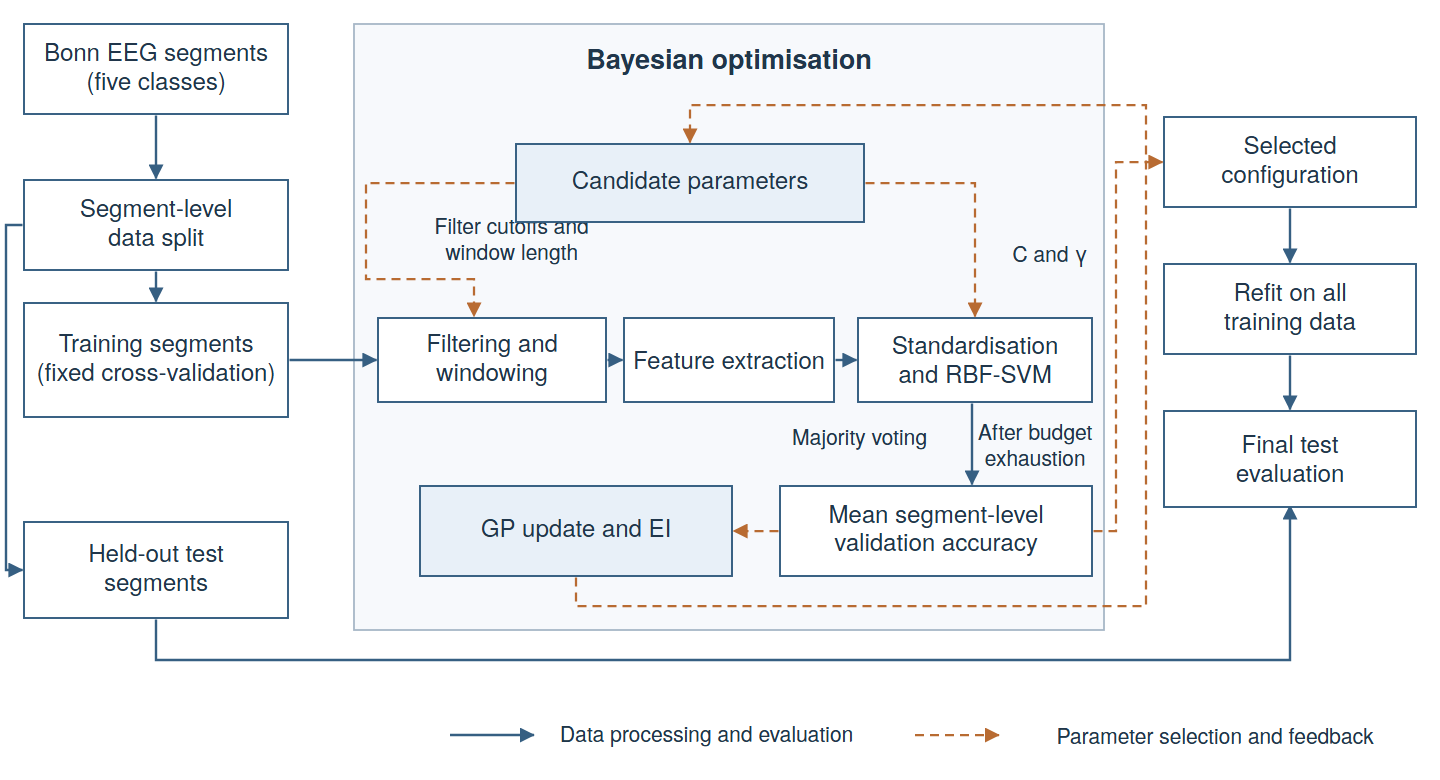
\includegraphics[width=\textwidth]
    {figures/implementation_overview.png}
    \caption{Implementation of the EEG classification
    framework. Blue solid arrows indicate data and model
    flow; orange dashed arrows indicate parameter control,
    selection and feedback. Held-out test segments are used
    only for final evaluation.}
    \label{fig:implementation-overview}
\end{figure}


\section{Dataset and Experimental Setup}
\label{sec:experimental-setup}

The experiments use a common classification procedure
to compare parameter-selection methods. This requires
a defined prediction task, a consistent feature
representation and a validation score that remains
comparable when preprocessing changes. The following
subsections describe the data, the construction of
classifier inputs and the conditions used to evaluate
candidate configurations.


\subsection{Dataset and Classification Task}
\label{subsec:dataset-task}

The Bonn EEG dataset provides labelled single-channel
segments of equal length \cite{Andrzejak2001}.
These properties allow a common processing procedure
to be applied across recordings, without introducing
channel selection or variable recording lengths into
the parameter-search comparison.

The dataset contains five sets, denoted by Z, O, N, F
and S, with 100 segments in each set. The files used
in this study contain 4097 sample values per segment
at a sampling frequency of 173.61 Hz, corresponding
to approximately 23.6 seconds.
Table~\ref{tab:bonn-five-classes} summarises the
recording conditions.

\begin{table}[htbp]
    \centering
    \caption{Recording conditions and segment counts
    of the Bonn EEG dataset \cite{Andrzejak2001}.}
    \label{tab:bonn-five-classes}
    \renewcommand{\arraystretch}{1.2}
    \begin{tabular}{cp{0.62\textwidth}r}
        \hline
        Label & Recording condition & Segments \\
        \hline
        Z & Healthy subjects, eyes open & 100 \\
        O & Healthy subjects, eyes closed & 100 \\
        N & Interictal EEG from the hippocampal formation
            contralateral to the epileptogenic zone & 100 \\
        F & Interictal EEG within the epileptogenic zone & 100 \\
        S & Ictal EEG during seizure activity & 100 \\
        \hline
        \multicolumn{2}{l}{Total} & 500 \\
        \hline
    \end{tabular}
\end{table}

Sets Z and O contain scalp recordings from healthy
subjects, while N, F and S contain intracranial recordings
from patients with epilepsy. All five original labels
are retained. This preserves distinctions between the
healthy recording conditions and between the two
interictal sets, as well as the distinction between
seizure and non-seizure activity. Class recall and
confusion matrices are examined alongside overall
accuracy to identify which categories account for
the classification errors.

Each original segment is called a recording in this
chapter. A window is a shorter portion extracted
from a recording for feature calculation. The complete
dataset can be represented by a $500\times4097$ matrix,
with one class label per row. Window extraction produces
several classifier inputs from each recording, all
inheriting the original label. Recordings remain the
units of data partitioning and final evaluation.



\subsection{Data Partitioning and Validation}
\label{subsec:data-partitioning}

Parameter search repeatedly uses validation scores to choose configurations.
A separate test set is therefore reserved to assess the selected configuration
on recordings that did not guide that search. A stratified 80\%--20\% split
produces 400 training and 100 test recordings, with 80 and 20 recordings per
class, respectively. This allocation retains most data for fitting and internal
validation while including every class in the final assessment. The split
proportion is a fixed experimental setting, rather than a ratio shown to be
optimal for this dataset.

The split precedes window extraction. Windows from one recording share signal
information and are kept together to avoid placing portions of the same
recording in both fitting and evaluation sets. Candidate configurations are
evaluated by five-fold stratified group cross-validation within the training
set, using the original recording identifier as the group. This combines
performance over several internal partitions, reducing dependence on a single
training--validation split. Five folds require five classifier fits per
candidate; no comparison establishing an optimal fold count is claimed.

\begin{table}[htbp]
\centering
\caption{Data partitioning and validation settings.}
\label{tab:data-validation-settings}
\renewcommand{\arraystretch}{1.15}
\begin{tabular}{lp{0.54\textwidth}}
\hline
Setting & Specification \\
\hline
Outer split & Stratified 80\% training, 20\% testing \\
Training and test sizes & 400 and 100 original recordings \\
Main comparison seed & 42 \\
Internal validation & Five-fold StratifiedGroupKFold \\
Grouping unit & Original recording, before window extraction \\
Fold allocation & Fixed within a run; shared across compared methods \\
Window prediction aggregation & Majority voting per recording \\
Selection score & Mean recording-level validation accuracy \\
Final assessment & Accuracy, class recall, macro-F1 and confusion matrix \\
\hline
\end{tabular}
\end{table}

Fold assignments are constructed at recording level and remain fixed as window
duration changes. Consequently, different configurations are evaluated on the
same validation recordings despite producing different numbers of windows.
Feature standardisation is fitted only on the training windows of each fold
and is then applied to its validation windows. This is necessary because the
features have different numerical scales, which otherwise affect RBF distances;
fitting the scaler within each fold also prevents validation information from
entering the fitted transformation. The classifier uses the same training
portion, with \texttt{class\_weight='balanced'} in all comparisons.

Window predictions are combined by majority vote to obtain one prediction per
recording. Ties are resolved by the smallest encoded label, with the order
Z, O, N, F and S. Recording-level scoring retains the original prediction unit
when window duration changes. The unweighted mean of the five fold accuracies
is returned as the selection score; its negative is supplied to the minimising
BO interface. Overall accuracy is complemented by class recall and confusion
matrices because an aggregate score can hide uneven class performance.

The highest-scoring evaluated configuration is selected, after which its
scaler and SVM are refitted on all training data. Its fixed preprocessing and
fitted scaler are then applied to the test recordings. The test set is not
used to choose candidates within that run. This is a held-out-recording
evaluation, not evidence of subject-independent performance. Moreover,
cross-validation scores repeatedly used during search are selection scores,
not independent estimates of final generalisation performance.

\subsection{Preprocessing and Feature Representation}
\label{subsec:preprocessing-features}

Changing the input frequency content changes the features presented to the
classifier. Filtering is therefore included in the search rather than fixed
independently of classification. The implementation applies a Butterworth
band-pass designed with \texttt{order=4}, represented as second-order sections
and applied forward and backward to each complete recording. Filtering before
windowing avoids introducing a separate filter boundary at every window.
Non-overlapping windows are then extracted using the nearest integer number
of samples to the requested duration; an incomplete trailing window is
discarded. Window duration controls both the time scale described by a feature
vector and the number of vectors available for fitting. Non-overlap limits
repeated use of the same samples across adjacent windows.

A supplementary descriptive PSD analysis was performed after the main search,
using only its 400 training recordings (seed 42; 80 per class).
Figure~\ref{fig:training-psd} summarises the unfiltered spectra. The O-class mean
has a peak near 11.2 Hz, and narrow peaks are visible near 50 Hz. These
observations describe the available signals; they do not identify the origin
of a peak, show that all high-frequency components are noise, or establish
classification-optimal filter cutoffs. In particular, this later analysis is
not presented as the original basis for the search endpoints.

\begin{figure}[htbp]
\centering
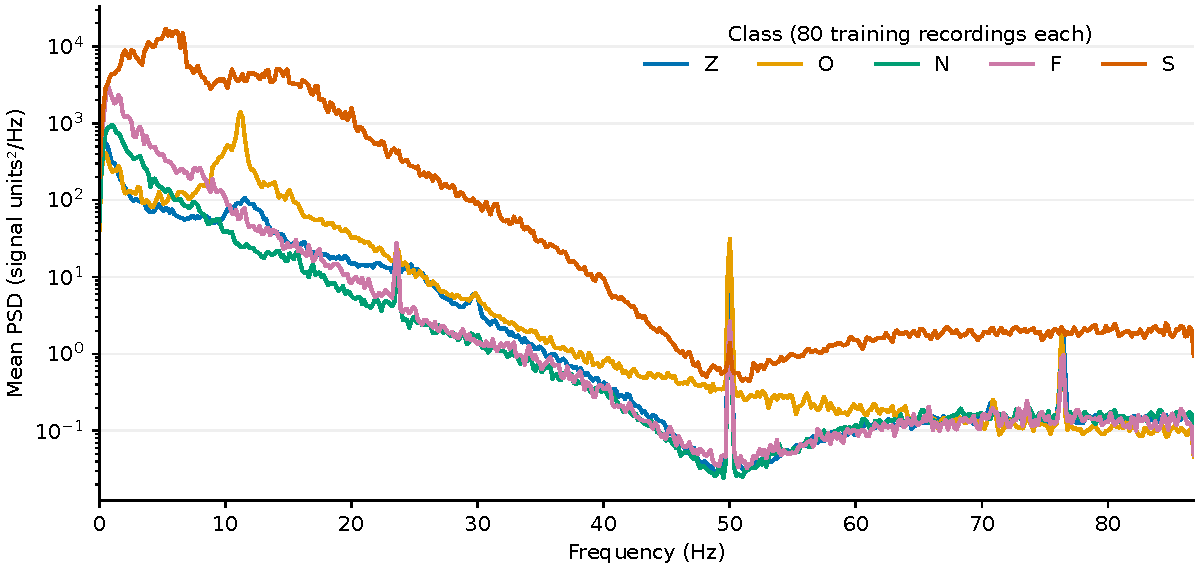
\includegraphics[width=\textwidth]{figures/training_class_mean_psd.pdf}
\caption{Class-wise mean PSD of the unfiltered training recordings (seed 42).
Welch estimates use a 1024-sample Hann window, 50\% overlap and constant
detrending. Recording spectra are averaged within each class before plotting
on a logarithmic vertical axis. These descriptive settings differ from those
used to calculate the window-level classifier features.}
\label{fig:training-psd}
\end{figure}

A fixed feature representation allows the comparison to focus on parameter
selection without simultaneously changing the feature set. Wavelet-based EEG
representations have been used by Subasi~\cite{Subasi2007}; relative spectral
powers, band ratios, statistical moments, Hjorth parameters and wavelet
energies also appear in seizure research~\cite{SeizurePredictionForecasting2024}.
These studies provide precedents for feature categories, not evidence that the
present combination of 55 columns, its precise bands or its implementation
settings are optimal.

\begin{table}[htbp]
\centering
\caption{Fixed window-level feature representation used in the main experiments.}
\label{tab:feature-composition}
\renewcommand{\arraystretch}{1.15}
\begin{tabular}{lp{0.53\textwidth}r}
\hline
Group & Computed descriptors & Columns \\
\hline
Spectral power & Absolute and relative power in five fixed bands & 10 \\
Band ratios & Six predefined power ratios & 6 \\
Statistics & Amplitude, distribution and waveform descriptors & 13 \\
Entropy & Amplitude-histogram, spectral and approximate entropy & 3 \\
Hjorth & Activity, mobility and complexity & 3 \\
Wavelet & Five summaries of each of four coefficient groups & 20 \\
\hline
Total & Fixed implementation-specific representation & 55 \\
\hline
\end{tabular}
\end{table}

The fixed spectral bands are 0.5--4, 4--8, 8--13, 13--30 and 30--40 Hz.
Changing the filter settings changes their measured powers without changing
these band definitions. Statistical descriptors summarise amplitudes and
waveform variation, while entropy and Hjorth measures add descriptors of
regularity and temporal variation. Wavelet features use db4 with three
decomposition levels, producing $A_3,D_3,D_2,D_1$. Energy, relative energy,
coefficient entropy, mean and standard deviation from each group give
20 columns. The wavelet and decomposition depth are fixed implementation
choices; the present comparison does not establish their superiority over
other choices. The complete representation is an $n\times55$ matrix for
$n$ windows. Its columns are not claimed to be independent or optimally selected.

\begin{table}[htbp]
\centering
\caption{Feature calculation settings retained in the reported experiments.}
\label{tab:feature-calculation-settings}
\renewcommand{\arraystretch}{1.15}
\begin{tabular}{lp{0.65\textwidth}}
\hline
Calculation & Implementation \\
\hline
Window PSD & Welch; \texttt{nperseg=min(256, window samples)}; remaining options use the installed SciPy defaults \\
Band power & Trapezoidal integration over frequency points in $[f_1,f_2)$; relative powers use the sum of the five band powers \\
Ratios & $\delta/\theta$, $\theta/\alpha$, $\alpha/\beta$, $\beta/\gamma$, $(\delta+\theta)/(\alpha+\beta)$, and $\gamma/\mathrm{total}$ \\
Statistics & Mean, standard deviation, variance, maximum, minimum, median, range, RMS, line length, skewness, kurtosis, energy and mean-centred zero crossings \\
Entropy & 32-bin amplitude histogram; normalised PSD; approximate entropy with $m=2$ and tolerance $0.2$ times the standard deviation of the evaluated sequence \\
Approximate entropy & At most 80 uniformly selected window samples; this computational approximation is fixed across methods \\
Wavelet & db4, three levels, default PyWavelets boundary extension \\
Numerical ratios & Denominators include a small $10^{-12}$ stabiliser \\
\hline
\end{tabular}
\end{table}

The short-window spectral features require cautious interpretation. A 0.5 Hz
oscillation has a two-second period, longer than the shortest one-second
classification window. Even for longer windows, the 256-sample Welch cap
corresponds to approximately 1.47 seconds and frequency-bin spacing of about
0.68 Hz. Thus, longer classification windows do not automatically provide
finer spectral spacing under this implementation. Classification utility does
not by itself establish stable low-frequency power estimation. This is a
limitation of the retained feature settings that warrants a separate check
of window duration and spectral estimation before any revised protocol is adopted.

\subsection{Search Domain and Numerical Settings}
\label{subsec:search-domain}

Each configuration contains the two filter cutoffs, window duration and the
RBF-SVM parameters $C$ and $\gamma$. Table~\ref{tab:search-domain} reports the
domain used in the completed main comparison. Its endpoints are empirical
project settings: there is no documented derivation of these exact values
from a publication, PSD analysis or systematic preliminary study. The
considerations below explain what is varied within this domain; they do not
establish why these endpoints are preferable to neighbouring alternatives.

\begin{table}[htbp]
\centering
\caption{Search domain retained for the main comparison. All exact endpoints
are empirical project settings, not validated optimal bounds.}
\label{tab:search-domain}
\renewcommand{\arraystretch}{1.15}
\begin{tabular}{lll}
\hline
Parameter & Range & Main-comparison representation \\
\hline
Lower cutoff $f_{\mathrm{low}}$ & $[0.5,5]$ Hz & Linear; uniform random sampling \\
Upper cutoff $f_{\mathrm{high}}$ & $[30,60]$ Hz & Linear; uniform random sampling \\
Window duration $T$ & $[1,5]$ s & Linear; uniform random sampling \\
SVM penalty $C$ & $[0.1,100]$ & Logarithmic; log-uniform random sampling \\
RBF parameter $\gamma$ & $[10^{-4},1]$ & Logarithmic; log-uniform random sampling \\
\hline
\end{tabular}
\end{table}

The cutoff intervals allow classification to be compared under different
degrees of low- and high-frequency attenuation. The window interval produces
approximately 4--23 complete windows per recording and examines several local
time scales. These properties do not justify excluding a 0.5-second window,
windows longer than five seconds, or other cutoff values. In particular,
60 Hz is a search endpoint, not an established physiological threshold or
a frequency justified by the later PSD plot.

The SVM parameters span multiple orders of magnitude, so logarithmic search
avoids concentrating independent samples at the numerically large end of
each interval. Hsu et al.~\cite{HsuSVMGuide} recommend validation-based search
over exponentially spaced values and give example grids
$C=2^{-5},2^{-3},\ldots,2^{15}$ and
$\gamma=2^{-15},2^{-13},\ldots,2^3$.
This supports the search strategy, but not the narrower exact ranges used
here. A future continuous log-scale search over those wider endpoints would
be an adaptation of that grid-search example and a change to the experimental
protocol, rather than a description of the present results.

\subsection{Comparison Conditions and Evaluation Budget}
\label{subsec:comparison-conditions}

The fixed reference configuration represents classification without automated
parameter selection. Random search measures the benefit of evaluating multiple
independently sampled configurations, while BO additionally uses earlier
parameter--score observations to choose subsequent candidates. Comparing BO
with random search therefore examines adaptive selection under a common
evaluation budget. Comparing either search with the fixed reference addresses
the combined benefit of additional evaluations and parameter selection.

\begin{table}[htbp]
\centering
\caption{Main comparison under the common data and feature protocol.}
\label{tab:method-budget}
\renewcommand{\arraystretch}{1.15}
\begin{tabular}{lcp{0.49\textwidth}}
\hline
Method & Evaluations & Parameter selection \\
\hline
Fixed reference & 1 & $f_{\mathrm{low}}=0.5$ Hz, $f_{\mathrm{high}}=40$ Hz, $T=2$ s, $C=10$, $\gamma=0.1$ \\
Random search & 50 & Independent uniform preprocessing and log-uniform SVM sampling \\
BO & 50 & 16 initial evaluations and 34 GP/EI-guided evaluations \\
\hline
\end{tabular}
\end{table}

The reference parameters are a fixed project configuration. No source has
been established that makes this combination a standard or commonly recommended
setting, and it is not treated as a strong manually optimised competitor.
Random search and BO use the same bounds, outer split, fixed folds,
feature definitions, scaling procedure and recording-level objective.
The main comparison uses seed 42. Variation across additional runs should
be reported only for methods and seeds actually completed; variation observed
in a separate mapping experiment does not establish repeated-run robustness
of the main method comparison.

One evaluation is one complete five-fold assessment of a candidate. The
reference therefore requires five SVM fits; each 50-evaluation search requires
250 fits before final refitting, provided all evaluations complete. This
controls objective-evaluation count, not elapsed time: window length changes
the number of training inputs, and BO adds surrogate-fitting and acquisition
costs. The 16 initial evaluations provide observations for the GP, leaving
34 evaluations for adaptive selection. Neither 16 nor 50 was demonstrated
to be optimal, and no retrospective computational-cost justification is
claimed. Conclusions are conditional on this resource allocation.

\subsection{Scope of the Comparison and Additional Checks}
\label{subsec:setup-scope}

The main comparison concerns the best configurations found within the stated
domain and budget. It does not establish a global optimum or adequate
coverage of all useful settings. In the saved seed-42 BO run, the selected
configuration reaches $f_{\mathrm{low}}=0.5$ Hz, $f_{\mathrm{high}}=60$ Hz and
$C=100$. These boundary values do not prove that performance improves beyond
the domain, but they motivate checking whether the conclusions depend on its
endpoints.

A supplementary boundary-sensitivity check is proposed, but has not been
performed as part of this revision. It should use only the existing training
recordings and fixed validation folds, with an explicitly specified set of
additional values around the active boundaries and all other settings held
constant. The purpose is to assess sensitivity of validation scores to the
domain, not to use test results to choose a new range. Such a check would be
reported as a subsequent analysis, not as the original source of the bounds.
If it leads to a revised search domain or feature calculation, both BO and
random search must be compared under the same revised protocol. Because the
original test results have already been inspected, any subsequent use of that
test set must be identified as a follow-up assessment rather than a fresh,
untouched confirmation.

After the main method comparison, alternative mappings of the preprocessing
parameters may be examined as an extension. Uniform, truncated-normal,
truncated-exponential and truncated-Gamma mappings are compared under otherwise
matched conditions, with one mapping per run. Their distribution settings
and results belong in the extension subsection, rather than being presented
as a second primary objective of the chapter.
